% ============================================================
% Question Bank: ch06-06 Angle Relationships (Modified — VA)
% Topic Title: Angle Relationships (VA SOL extended angle emphasis)
% CCSS: 7.G.B.5 (Modified for Virginia)
% Questions: 30 (18 MC + 7 SA + 5 Graphical)
% ============================================================

% --- Multiple Choice Questions (18) ---

\begin{practiceQuestion}{m-6-6-q01}{mc}
\begin{questionText}
Two angles are supplementary. One angle is $3x + 15$ and the other is $2x + 5$. What are the two angle measures?
\end{questionText}
\choiceA{$111°$ and $69°$}
\choiceB{$105°$ and $75°$}
\choiceC{$120°$ and $60°$}
\choiceD{$95°$ and $85°$}
\correctAnswer{A}
\explanation{$3x + 15 + 2x + 5 = 180$. Combine: $5x + 20 = 180$. Solve: $5x = 160$, $x = 32$. Angles: $3(32) + 15 = 111°$ and $2(32) + 5 = 69°$. Check: $111 + 69 = 180°$ \checkmark.}
\end{practiceQuestion}

\begin{practiceQuestion}{m-6-6-q02}{mc}
\begin{questionText}
Two vertical angles are $(4x - 10)°$ and $(2x + 30)°$. Find the angle measure.
\end{questionText}
\choiceA{$20°$}
\choiceB{$50°$}
\choiceC{$70°$}
\choiceD{$110°$}
\correctAnswer{C}
\explanation{Vertical angles are equal: $4x - 10 = 2x + 30$. Solve: $2x = 40$, $x = 20$. Angle: $4(20) - 10 = 70°$.}
\end{practiceQuestion}

\begin{practiceQuestion}{m-6-6-q03}{mc}
\begin{questionText}
Two lines intersect. One pair of vertical angles is $70°$. The supplementary angle to one of these is:
\end{questionText}
\choiceA{$20°$}
\choiceB{$70°$}
\choiceC{$110°$}
\choiceD{$290°$}
\correctAnswer{C}
\explanation{Supplementary to $70°$: $180° - 70° = 110°$.}
\end{practiceQuestion}

\begin{practiceQuestion}{m-6-6-q04}{mc}
\begin{questionText}
An angle is $20°$ more than $3$ times its complement. What is the angle?
\end{questionText}
\choiceA{$17.5°$}
\choiceB{$52.5°$}
\choiceC{$67.5°$}
\choiceD{$72.5°$}
\correctAnswer{D}
\explanation{Let complement $= x$. Angle $= 3x + 20$. Sum: $x + 3x + 20 = 90$. Combine: $4x = 70$, $x = 17.5°$. Angle: $3(17.5) + 20 = 72.5°$.}
\end{practiceQuestion}

\begin{practiceQuestion}{m-6-6-q05}{mc}
\begin{questionText}
Three angles meet at a point on a line: $(x + 20)°$, $(2x)°$, and $40°$. What is $x$?
\end{questionText}
\choiceA{$30$}
\choiceB{$40$}
\choiceC{$50$}
\choiceD{$60$}
\correctAnswer{B}
\explanation{Angles on a line sum to $180°$: $x + 20 + 2x + 40 = 180$. Combine: $3x + 60 = 180$. Solve: $3x = 120$, $x = 40$.}
\end{practiceQuestion}

\begin{practiceQuestion}{m-6-6-q06}{mc}
\begin{questionText}
Two complementary angles are $(5x - 10)°$ and $(3x + 4)°$. Find the larger angle.
\end{questionText}
\choiceA{$36°$}
\choiceB{$40°$}
\choiceC{$50°$}
\choiceD{$54°$}
\correctAnswer{C}
\explanation{$5x - 10 + 3x + 4 = 90$. Combine: $8x - 6 = 90$. Solve: $8x = 96$, $x = 12$. Angles: $5(12) - 10 = 50°$ and $3(12) + 4 = 40°$. Larger is $50°$.}
\end{practiceQuestion}

\begin{practiceQuestion}{m-6-6-q07}{mc}
\begin{questionText}
Two intersecting lines form four angles. If one angle is $x°$, the four angles in order around the intersection are:
\end{questionText}
\choiceA{$x°$, $x°$, $x°$, $x°$}
\choiceB{$x°$, $(180 - x)°$, $x°$, $(180 - x)°$}
\choiceC{$x°$, $(90 - x)°$, $x°$, $(90 - x)°$}
\choiceD{$x°$, $(360 - x)°$, $x°$, $x°$}
\correctAnswer{B}
\explanation{Vertical angles are equal ($x°$ and $x°$). Adjacent angles are supplementary: $180° - x°$. The pattern is $x$, $180-x$, $x$, $180-x$.}
\end{practiceQuestion}

\begin{practiceQuestion}{m-6-6-q08}{mc}
\begin{questionText}
Two supplementary angles have a ratio of $7:2$. What is the smaller angle?
\end{questionText}
\choiceA{$20°$}
\choiceB{$36°$}
\choiceC{$40°$}
\choiceD{$140°$}
\correctAnswer{C}
\explanation{$7x + 2x = 180$. So $9x = 180$ and $x = 20$. Smaller angle: $2(20) = 40°$. Larger: $7(20) = 140°$.}
\end{practiceQuestion}

\begin{practiceQuestion}{m-6-6-q09}{mc}
\begin{questionText}
Two vertical angles are $(6y + 8)°$ and $(4y + 24)°$. Find the supplementary angle to one of these vertical angles.
\end{questionText}
\choiceA{$56°$}
\choiceB{$124°$}
\choiceC{$128°$}
\choiceD{$132°$}
\correctAnswer{B}
\explanation{Vertical angles equal: $6y + 8 = 4y + 24$. Solve: $2y = 16$, $y = 8$. Vertical angle: $6(8) + 8 = 56°$. Supplementary: $180° - 56° = 124°$.}
\end{practiceQuestion}

\begin{practiceQuestion}{m-6-6-q10}{mc}
\begin{questionText}
An angle measures $(2x + 15)°$ and its supplement measures $(4x - 9)°$. Find $x$ and both angle measures.
\end{questionText}
\choiceA{$x = 29$; angles $73°$ and $107°$}
\choiceB{$x = 29$; angles $63°$ and $117°$}
\choiceC{$x = 25$; angles $65°$ and $115°$}
\choiceD{$x = 30$; angles $75°$ and $105°$}
\correctAnswer{A}
\explanation{$2x + 15 + 4x - 9 = 180$. Combine: $6x + 6 = 180$. Solve: $6x = 174$, $x = 29$. Angles: $2(29) + 15 = 73°$ and $4(29) - 9 = 107°$. Check: $73 + 107 = 180°$ \checkmark.}
\end{practiceQuestion}

\begin{practiceQuestion}{m-6-6-q11}{mc}
\begin{questionText}
An angle is supplementary to a $55°$ angle. Is the supplementary angle also complementary to any angle? If so, which?
\end{questionText}
\choiceA{No, a $125°$ angle cannot have a complement}
\choiceB{Yes, its complement is $35°$}
\choiceC{Yes, its complement is $55°$}
\choiceD{Yes, its complement is $65°$}
\correctAnswer{A}
\explanation{Supplement of $55°$ is $125°$. Complementary angles must be less than or equal to $90°$. Since $125° > 90°$, it has no complement.}
\end{practiceQuestion}

\begin{practiceQuestion}{m-6-6-q12}{mc}
\begin{questionText}
Two angles are both supplementary to the same angle. What must be true about those two angles?
\end{questionText}
\choiceA{They are complementary}
\choiceB{They are vertical}
\choiceC{They are equal}
\choiceD{They sum to $360°$}
\correctAnswer{C}
\explanation{If angle $A$ + angle $C$ $= 180$ and angle $B$ + angle $C$ $= 180$, then $A = B$. Two angles supplementary to the same angle are equal.}
\end{practiceQuestion}

\begin{practiceQuestion}{m-6-6-q13}{mc}
\begin{questionText}
Four angles meet at a point (not on a line). They measure $(2x)°$, $(3x)°$, $(4x)°$, and $(x + 40)°$. Find $x$.
\end{questionText}
\choiceA{$28$}
\choiceB{$32$}
\choiceC{$36$}
\choiceD{$40$}
\correctAnswer{B}
\explanation{Angles around a point sum to $360°$: $2x + 3x + 4x + x + 40 = 360$. Combine: $10x + 40 = 360$. Solve: $10x = 320$, $x = 32$.}
\end{practiceQuestion}

\begin{practiceQuestion}{m-6-6-q14}{mc}
\begin{questionText}
Angle $A$ and angle $B$ are vertical angles. Angle $A$ and angle $C$ are supplementary. If angle $B = 48°$, what is angle $C$?
\end{questionText}
\choiceA{$42°$}
\choiceB{$48°$}
\choiceC{$132°$}
\choiceD{$138°$}
\correctAnswer{C}
\explanation{Vertical: $A = B = 48°$. Supplementary: $C = 180° - 48° = 132°$.}
\end{practiceQuestion}

\begin{practiceQuestion}{m-6-6-q15}{mc}
\begin{questionText}
The complement of an angle is $15°$ less than the angle itself. What is the angle?
\end{questionText}
\choiceA{$37.5°$}
\choiceB{$45°$}
\choiceC{$52.5°$}
\choiceD{$75°$}
\correctAnswer{C}
\explanation{Let the angle be $x$. Complement: $90 - x$. Given: $90 - x = x - 15$. Solve: $90 + 15 = 2x$, $105 = 2x$, $x = 52.5°$.}
\end{practiceQuestion}

\begin{practiceQuestion}{m-6-6-q16}{mc}
\begin{questionText}
Two angles are supplementary. The larger is $3$ times the smaller. What is the larger angle?
\end{questionText}
\choiceA{$45°$}
\choiceB{$60°$}
\choiceC{$120°$}
\choiceD{$135°$}
\correctAnswer{D}
\explanation{Let smaller $= x$, larger $= 3x$. $x + 3x = 180$. So $4x = 180$ and $x = 45°$. Larger: $3(45) = 135°$.}
\end{practiceQuestion}

\begin{practiceQuestion}{m-6-6-q17}{mc}
\begin{questionText}
Angles $P$ and $Q$ are complementary. Angles $Q$ and $R$ are supplementary. If $P = 25°$, what is $R$?
\end{questionText}
\choiceA{$65°$}
\choiceB{$115°$}
\choiceC{$155°$}
\choiceD{$90°$}
\correctAnswer{B}
\explanation{$P + Q = 90$, so $Q = 90 - 25 = 65°$. $Q + R = 180$, so $R = 180 - 65 = 115°$.}
\end{practiceQuestion}

\begin{practiceQuestion}{m-6-6-q18}{mc}
\begin{questionText}
Two lines intersect. The four angles formed are $(3a + 10)°$, $(5a - 30)°$, $(3a + 10)°$, and $(5a - 30)°$. What is $a$?
\end{questionText}
\choiceA{$10$}
\choiceB{$15$}
\choiceC{$20$}
\choiceD{$25$}
\correctAnswer{D}
\explanation{Adjacent angles are supplementary: $(3a + 10) + (5a - 30) = 180$. Combine: $8a - 20 = 180$. Solve: $8a = 200$, $a = 25$.}
\end{practiceQuestion}

% --- Short Answer Questions (7) ---

\begin{practiceQuestion}{m-6-6-q19}{sa}
\begin{questionText}
Two vertical angles are $(9x - 4)°$ and $(7x + 12)°$. Find $x$ and the angle measure.
\end{questionText}
\correctAnswer{$x = 8$; the angles are $68°$}
\explanation{$9x - 4 = 7x + 12$. Subtract $7x$: $2x - 4 = 12$. Add $4$: $2x = 16$. $x = 8$. Angle: $9(8) - 4 = 68°$.}
\end{practiceQuestion}

\begin{practiceQuestion}{m-6-6-q20}{sa}
\begin{questionText}
Angles $A$, $B$, and $C$ meet on a straight line. $A = (3x + 5)°$, $B = (2x + 10)°$, $C = (x + 15)°$. Find all three angle measures.
\end{questionText}
\correctAnswer{$A = 80°$, $B = 60°$, $C = 40°$}
\explanation{$3x + 5 + 2x + 10 + x + 15 = 180$. Combine: $6x + 30 = 180$. Solve: $6x = 150$, $x = 25$. Angles: $3(25)+5=80°$, $2(25)+10=60°$, $25+15=40°$. Check: $80+60+40=180°$ \checkmark.}
\end{practiceQuestion}

\begin{practiceQuestion}{m-6-6-q21}{sa}
\begin{questionText}
The supplement of an angle is $40°$ more than twice the angle. Find the angle.
\end{questionText}
\correctAnswer{$\frac{140}{3}°$ or approximately $46.7°$}
\explanation{Let angle $= x$. Supplement $= 180 - x$. Given: $180 - x = 2x + 40$. Solve: $180 - 40 = 3x$, $140 = 3x$, $x = \frac{140}{3} \approx 46.7°$.}
\end{practiceQuestion}

\begin{practiceQuestion}{m-6-6-q22}{sa}
\begin{questionText}
Two complementary angles are in the ratio $3:7$. Find both angles.
\end{questionText}
\correctAnswer{$27°$ and $63°$}
\explanation{$3x + 7x = 90$. $10x = 90$. $x = 9$. Angles: $3(9) = 27°$ and $7(9) = 63°$.}
\end{practiceQuestion}

\begin{practiceQuestion}{m-6-6-q23}{sa}
\begin{questionText}
Angle $X$ is vertical to angle $Y$. Angle $Y$ is complementary to a $35°$ angle. Angle $X$ is supplementary to angle $Z$. Find angle $Z$.
\end{questionText}
\correctAnswer{$125°$}
\explanation{$Y$ is complementary to $35°$: $Y = 90 - 35 = 55°$. Vertical: $X = Y = 55°$. Supplementary: $Z = 180 - 55 = 125°$.}
\end{practiceQuestion}

\begin{practiceQuestion}{m-6-6-q24}{sa}
\begin{questionText}
Two angles are equal and supplementary. A third angle is complementary to one of them. What is the third angle?
\end{questionText}
\correctAnswer{No such angle exists (or: it is impossible)}
\explanation{Equal supplementary angles: $x + x = 180$, so $x = 90°$. The complement of $90°$ would be $0°$, which is not a valid angle. No complement exists.}
\end{practiceQuestion}

\begin{practiceQuestion}{m-6-6-q25}{sa}
\begin{questionText}
Five angles meet at a point: $50°$, $(2x)°$, $70°$, $(3x - 10)°$, and $80°$. Find $x$.
\end{questionText}
\correctAnswer{$x = 34$}
\explanation{$50 + 2x + 70 + 3x - 10 + 80 = 360$. Combine: $5x + 190 = 360$. Solve: $5x = 170$, $x = 34$.}
\end{practiceQuestion}

% --- Graphical Questions (3 GMC + 2 GSA) ---

\begin{practiceQuestion}{m-6-6-q26}{gmc}
\begin{questionText}
Two lines intersect as shown. Find the value of $x$.

\begin{center}
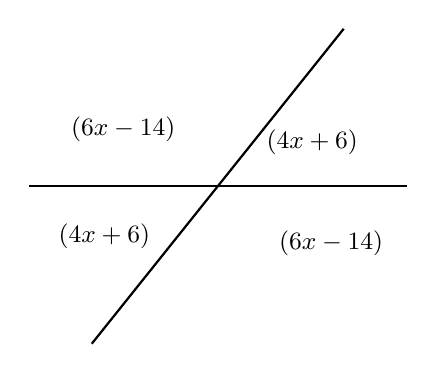
\begin{tikzpicture}[scale=0.8]
  \draw[thick] (-3,0) -- (3,0);
  \draw[thick] (-2,-2.5) -- (2,2.5);
  \node at (1.5,0.7) {\small $(4x+6)°$};
  \node at (-1.8,-0.8) {\small $(4x+6)°$};
  \node at (-1.5,0.9) {\small $(6x-14)°$};
  \node at (1.8,-0.9) {\small $(6x-14)°$};
\end{tikzpicture}
\end{center}
\end{questionText}
\choiceA{$10$}
\choiceB{$14$}
\choiceC{$18.8$}
\choiceD{$20$}
\correctAnswer{C}
\explanation{Adjacent angles are supplementary: $(4x+6) + (6x-14) = 180$. Combine: $10x - 8 = 180$. Solve: $10x = 188$, $x = 18.8$.}
\end{practiceQuestion}

\begin{practiceQuestion}{m-6-6-q27}{gmc}
\begin{questionText}
In the diagram, angles $1$ through $4$ are formed by two intersecting lines. Angle $1 = 63°$. What is the sum of angles $2$ and $4$?

\begin{center}
\begin{tikzpicture}[scale=0.8]
  \draw[thick] (-3,0) -- (3,0);
  \draw[thick] (-1.5,-2.5) -- (1.5,2.5);
  \node at (0,0) [below left,xshift=-2pt,yshift=-2pt] {};
  \node at (1.3,0.7) {\small $\angle 1$};
  \node at (-1.3,0.7) {\small $\angle 2$};
  \node at (-1.3,-0.7) {\small $\angle 3$};
  \node at (1.3,-0.7) {\small $\angle 4$};
  \node[right] at (2.5,1) {\small $\angle 1 = 63°$};
\end{tikzpicture}
\end{center}
\end{questionText}
\choiceA{$126°$}
\choiceB{$180°$}
\choiceC{$234°$}
\choiceD{$297°$}
\correctAnswer{C}
\explanation{$\angle 3$ is vertical to $\angle 1$: $\angle 3 = 63°$. $\angle 2$ is supplementary to $\angle 1$: $\angle 2 = 117°$. $\angle 4$ is vertical to $\angle 2$: $\angle 4 = 117°$. Sum: $\angle 2 + \angle 4 = 117 + 117 = 234°$.}
\end{practiceQuestion}

\begin{practiceQuestion}{m-6-6-q28}{gmc}
\begin{questionText}
In the diagram, the three angles on a straight line are labeled. Which equation can be used to find $x$?

\begin{center}
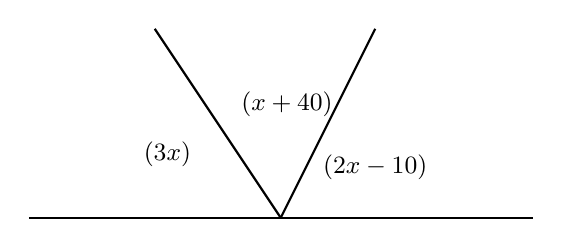
\begin{tikzpicture}[scale=0.8]
  \draw[thick] (-4,0) -- (4,0);
  \draw[thick] (0,0) -- (-2,3);
  \draw[thick] (0,0) -- (1.5,3);
  \node at (-1.8,1) {\small $(3x)°$};
  \node at (0.1,1.8) {\small $(x+40)°$};
  \node at (1.5,0.8) {\small $(2x-10)°$};
\end{tikzpicture}
\end{center}
\end{questionText}
\choiceA{$3x + (x + 40) + (2x - 10) = 90$}
\choiceB{$3x + (x + 40) + (2x - 10) = 180$}
\choiceC{$3x + (x + 40) + (2x - 10) = 360$}
\choiceD{$3x = (x + 40) + (2x - 10)$}
\correctAnswer{B}
\explanation{Angles on a straight line sum to $180°$. The equation is $3x + (x + 40) + (2x - 10) = 180$.}
\end{practiceQuestion}

\begin{practiceQuestion}{m-6-6-q29}{gsa}
\begin{questionText}
Two lines intersect as shown. Find all four angle measures.

\begin{center}
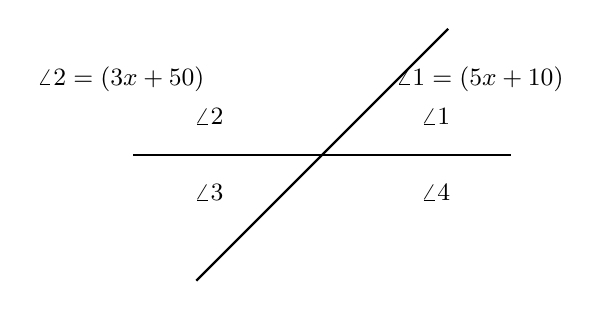
\begin{tikzpicture}[scale=0.8]
  \draw[thick] (-3,0) -- (3,0);
  \draw[thick] (-2,-2) -- (2,2);
  \node at (1.8,0.6) {\small $\angle 1$};
  \node at (-1.8,0.6) {\small $\angle 2$};
  \node at (-1.8,-0.6) {\small $\angle 3$};
  \node at (1.8,-0.6) {\small $\angle 4$};
  \node at (2.5,1.2) {\small $\angle 1 = (5x+10)°$};
  \node at (-3.2,1.2) {\small $\angle 2 = (3x+50)°$};
\end{tikzpicture}
\end{center}
\end{questionText}
\correctAnswer{$\angle 1 = 85°$, $\angle 2 = 95°$, $\angle 3 = 85°$, $\angle 4 = 95°$}
\explanation{$\angle 1 + \angle 2 = 180$: $(5x+10) + (3x+50) = 180$. Combine: $8x + 60 = 180$. Solve: $8x = 120$, $x = 15$. $\angle 1 = 5(15)+10 = 85°$, $\angle 2 = 3(15)+50 = 95°$. Vertical: $\angle 3 = 85°$, $\angle 4 = 95°$.}
\end{practiceQuestion}

\begin{practiceQuestion}{m-6-6-q30}{gsa}
\begin{questionText}
In the diagram below, four angles meet at a point. Find the value of $y$ and all four angle measures.

\begin{center}
\begin{tikzpicture}[scale=0.8]
  \draw[thick] (-3,0) -- (3,0);
  \draw[thick] (0,-3) -- (0,3);
  \draw (0.4,0) arc[start angle=0,end angle=90,radius=0.4];
  \node at (1.5,1.2) {\small $(2y+10)°$};
  \node at (-1.5,1.2) {\small $(3y - 5)°$};
  \node at (-1.5,-1.2) {\small $(2y+10)°$};
  \node at (1.5,-1.2) {\small $(3y-5)°$};
\end{tikzpicture}
\end{center}
\end{questionText}
\correctAnswer{$y = 35$; angles are $80°$, $100°$, $80°$, $100°$}
\explanation{Adjacent angles are supplementary: $(2y+10) + (3y-5) = 180$. Combine: $5y + 5 = 180$. Solve: $5y = 175$, $y = 35$. Angles: $2(35)+10 = 80°$ and $3(35)-5 = 100°$. The four angles: $80°$, $100°$, $80°$, $100°$. Check: $80+100+80+100 = 360°$ \checkmark.}
\end{practiceQuestion}
